\documentclass[11pt,a4paper]{article}

% ===================== PACKAGES =====================
\usepackage[margin=2.2cm,top=2.6cm,bottom=2.8cm]{geometry}
\usepackage{fontspec}
\usepackage{xcolor}
\usepackage{graphicx}
\usepackage{booktabs}
\usepackage{longtable}
\usepackage{array}
\usepackage{colortbl}
\usepackage[most]{tcolorbox}
\usepackage{titlesec}
\usepackage{fancyhdr}
\usepackage{enumitem}
\usepackage{hyperref}
\usepackage{tikz}
\usepackage{multicol}
\usepackage{caption}

\tcbuselibrary{skins,breakable}

% ===================== FONTS =====================
\setmainfont{Liberation Sans}
\newfontfamily\monofont{DejaVu Sans Mono}

% ===================== COLORS =====================
\definecolor{navy}{HTML}{16324F}
\definecolor{navydark}{HTML}{0D2136}
\definecolor{teal}{HTML}{1A936F}
\definecolor{tealdark}{HTML}{146C52}
\definecolor{greenok}{HTML}{2E8B57}
\definecolor{critred}{HTML}{C0392B}
\definecolor{highorange}{HTML}{E07B39}
\definecolor{medyellow}{HTML}{D4A017}
\definecolor{lowgray}{HTML}{6C7A89}
\definecolor{lightbg}{HTML}{F4F7F9}
\definecolor{panelbg}{HTML}{EDF2F5}
\definecolor{bodytext}{HTML}{233241}
\definecolor{rulegray}{HTML}{C7D0D8}
\definecolor{termbg}{HTML}{0B0F14}

\color{bodytext}

% ===================== SECTION STYLING =====================
\titleformat{\section}
  {\normalfont\Large\bfseries\color{navy}}
  {\thesection}{0.5em}{}
\titlespacing*{\section}{0pt}{1.6em}{0.9em}
\titleformat{\subsection}
  {\normalfont\large\bfseries\color{tealdark}}
  {\thesubsection}{0.5em}{}
\titlespacing*{\subsection}{0pt}{1.2em}{0.6em}

% ===================== HEADER/FOOTER =====================
\pagestyle{fancy}
\fancyhf{}
\renewcommand{\headrulewidth}{0.6pt}
\renewcommand{\headrule}{\hbox to\headwidth{\color{rulegray}\leaders\hrule height \headrulewidth\hfill}}
\fancyhead[L]{\small\color{lowgray}Penetration Testing Report --- Metasploitable2}
\fancyhead[R]{\small\color{lowgray}CONFIDENTIAL}
\fancyfoot[L]{\small\color{lowgray}Prepared by Eyad El-Taher}
\fancyfoot[R]{\small\color{lowgray}Page \thepage\ of \pageref{LastPage}}

% ===================== HYPERLINKS =====================
\hypersetup{
  colorlinks=true,
  linkcolor=tealdark,
  urlcolor=tealdark,
  citecolor=tealdark,
  pdftitle={Penetration Testing Report - Metasploitable2},
  pdfauthor={Eyad El-Taher}
}

% ===================== CUSTOM ENVIRONMENTS =====================

% Severity pill macro
\newcommand{\sev}[1]{%
  \ifcase#1
    \colorbox{lowgray}{\textcolor{white}{\small\textbf{ INFO }}}%
  \or
    \colorbox{lowgray}{\textcolor{white}{\small\textbf{ LOW }}}%
  \or
    \colorbox{medyellow}{\textcolor{white}{\small\textbf{ MEDIUM }}}%
  \or
    \colorbox{highorange}{\textcolor{white}{\small\textbf{ HIGH }}}%
  \or
    \colorbox{critred}{\textcolor{white}{\small\textbf{ CRITICAL }}}%
  \fi
}

% Evidence / terminal screenshot box (#1 = evidence number, #2 = caption)
\newtcolorbox{evidence}[2]{
  breakable,
  enhanced,
  colback=termbg,
  colframe=rulegray,
  boxrule=0.4pt,
  arc=2pt,
  top=6pt, bottom=6pt, left=6pt, right=6pt,
  fonttitle=\bfseries\sffamily\small,
  coltitle=white,
  colbacktitle=navydark,
  title={Evidence #1 --- #2},
  attach boxed title to top left={xshift=6pt,yshift=-2pt},
  boxed title style={colback=navydark,arc=2pt,boxrule=0pt},
}

% Info / callout panel
\newtcolorbox{panel}[1][]{
  colback=panelbg,
  colframe=rulegray,
  boxrule=0.5pt,
  arc=2pt,
  left=10pt, right=10pt, top=8pt, bottom=8pt,
  #1
}

% Recommendation box
\newtcolorbox{recbox}[1]{
  colback=white,
  colframe=teal,
  boxrule=0.8pt,
  arc=2pt,
  left=10pt, right=10pt, top=7pt, bottom=8pt,
  fonttitle=\bfseries\sffamily,
  coltitle=white,
  colbacktitle=teal,
  title={#1},
}

\newcolumntype{L}[1]{>{\raggedright\arraybackslash}p{#1}}

\usepackage{lastpage}

% ===================== DOCUMENT =====================
\begin{document}

% ---------- TITLE PAGE ----------
\begin{titlepage}
\newgeometry{margin=0cm}
\noindent
\begin{tikzpicture}[remember picture, overlay]
  \fill[navy] (current page.north west) rectangle ([yshift=-6.8cm]current page.north east);
  \fill[teal] ([yshift=-6.8cm]current page.north west) rectangle ([yshift=-6.95cm]current page.north east);
\end{tikzpicture}

\begin{minipage}[t][6.8cm][c]{\paperwidth}
\hspace{2.4cm}
\begin{minipage}{0.88\paperwidth}
\raggedright\hyphenpenalty=10000\exhyphenpenalty=10000
\color{white}
{\small\bfseries\sffamily\color{teal!60!white} PENETRATION TESTING ENGAGEMENT}\\[0.4em]
{\fontsize{29}{34}\selectfont\bfseries\sffamily Network Penetration Test Report}\\[0.3em]
{\Large\sffamily Metasploitable 2 --- Internal Lab Assessment}
\end{minipage}
\end{minipage}

\vspace{2.4cm}

\hspace{2.4cm}
\begin{minipage}{0.8\paperwidth}
\renewcommand{\arraystretch}{1.6}
\begin{tabular}{L{4.2cm} L{9.5cm}}
\textbf{\color{navy}Prepared by} & Eyad El-Taher \\
\textbf{\color{navy}Engagement type} & Internal network penetration test (lab / training environment) \\
\textbf{\color{navy}Target} & Metasploitable2 --- \texttt{192.168.56.101} \\
\textbf{\color{navy}Network scope} & \texttt{192.168.56.0/24} \\
\textbf{\color{navy}Assessment window} & 29 August 2026, 01:40 -- 03:14 (+03:00) \\
\textbf{\color{navy}Classification} & Confidential --- for training/educational purposes only \\
\end{tabular}
\end{minipage}

\vfill

\hspace{2.4cm}
\begin{minipage}{0.8\paperwidth}
\begin{panel}
\small
This report documents a black-box network penetration test performed against an isolated, intentionally vulnerable lab virtual machine (Metasploitable2) as part of a hands-on training exercise. No production systems, third-party assets, or externally routable hosts were in scope. All activity was carried out inside a local, host-only virtual network (\texttt{192.168.56.0/24}) with no internet-facing exposure.
\end{panel}
\end{minipage}

\restoregeometry
\end{titlepage}

\tableofcontents
\thispagestyle{empty}
\clearpage

% ======================================================
\section{Target Information}
% ======================================================

\begin{panel}
\renewcommand{\arraystretch}{1.5}
\begin{tabular}{L{4.5cm} L{9.7cm}}
\textbf{Target name} & Metasploitable2 (deliberately vulnerable Linux VM) \\
\textbf{Target IP address} & \texttt{192.168.56.101} \\
\textbf{Network / scope} & \texttt{192.168.56.0/24} (host-only virtual adapter) \\
\textbf{Attacking host} & arch Linux workstation on the same host-only segment \\
\textbf{Engagement window} & 29 August 2026, 01:40 -- 03:14 (+03:00) \\
\textbf{Testing style} & Unauthenticated, black-box network penetration test \\
\textbf{Rules of engagement} & Isolated lab network; no production or third-party systems in scope \\
\end{tabular}
\end{panel}

\subsection*{Objectives}
\begin{itemize}[leftmargin=1.4em]
\item Perform network discovery across the \texttt{192.168.56.0/24} subnet to identify live hosts.
\item Enumerate open ports and fingerprint running services on the target.
\item Identify outdated software versions and map them to known CVEs.
\item Validate exploitability of high-risk findings (e.g. the vsftpd 2.3.4 backdoor) and demonstrate credential-based attacks.
\item Document misconfigurations and provide prioritised, actionable remediation guidance.
\end{itemize}

% ======================================================
\section{Reconnaissance Results}
% ======================================================

\subsection{Host Discovery}
A ping sweep (\texttt{nmap -sn}) was run against the full \texttt{192.168.56.0/24} subnet to enumerate live hosts before any port-level scanning took place.

\begin{evidence}{1}{Host discovery sweep and start of service scan --- \texttt{nmap -sn} / \texttt{nmap -A 192.168.56.101}}
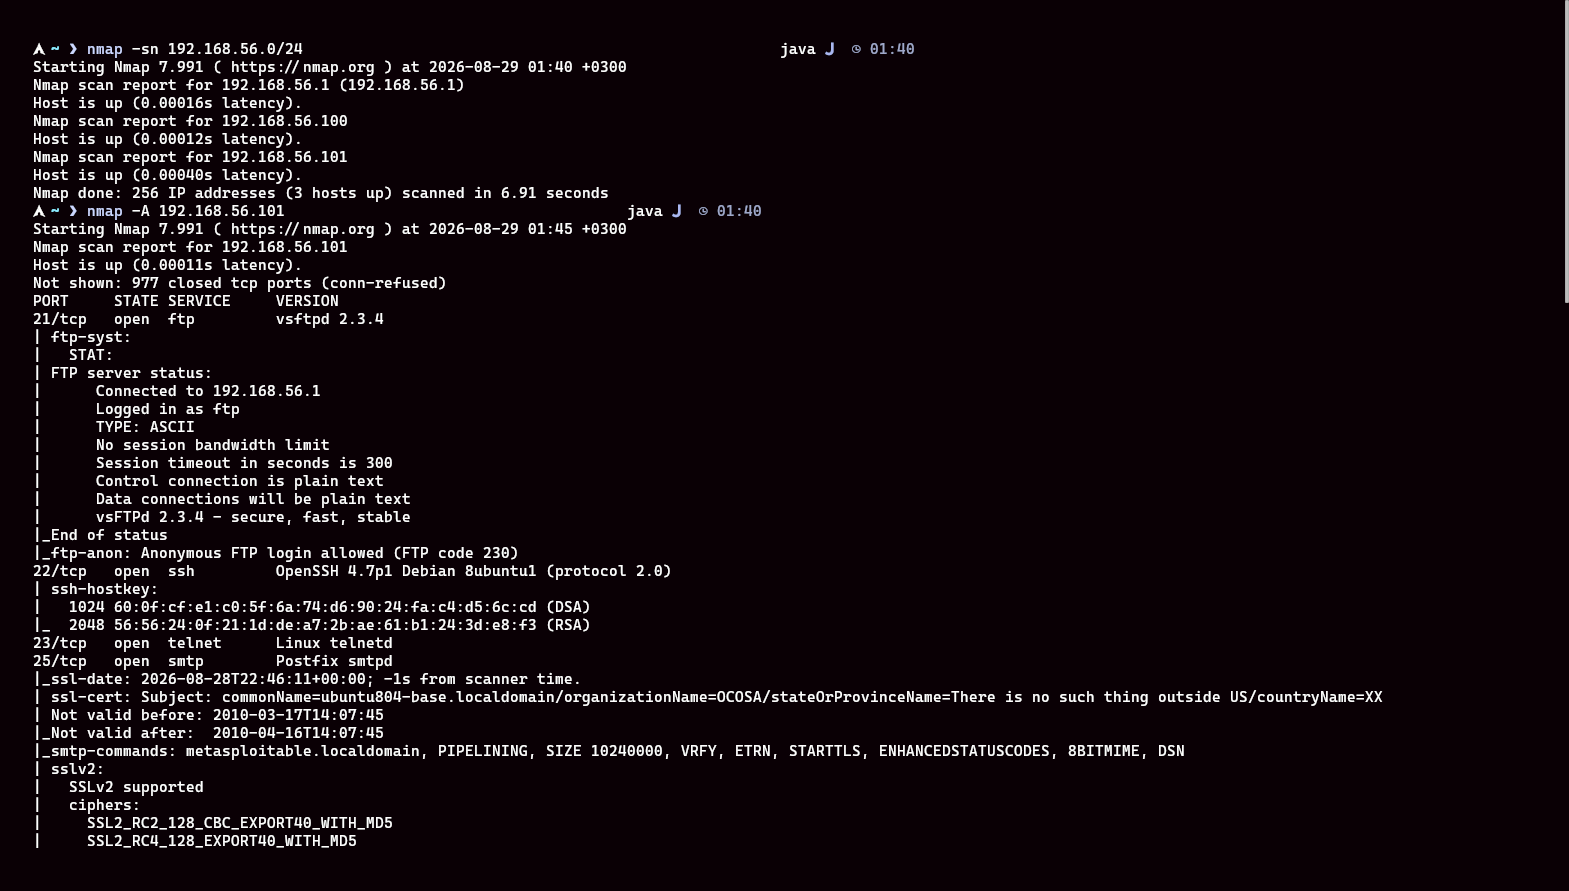
\includegraphics[width=\linewidth]{images/command1.jpg}
\end{evidence}

Three hosts responded: the host-only gateway/adapter (\texttt{.1}), a secondary lab host (\texttt{.100}), and the assessment target (\texttt{.101}). Full details are in Section~3.

\subsection{Service and Version Scan}
An aggressive scan (\texttt{nmap -A}) was then run against the target to enumerate open ports, detect service versions, pull banners, and run default NSE scripts. The scan output (continued from Evidence~1 above) is shown across the two captures below.

\begin{evidence}{2}{Aggressive scan continued --- ports 25--3306}
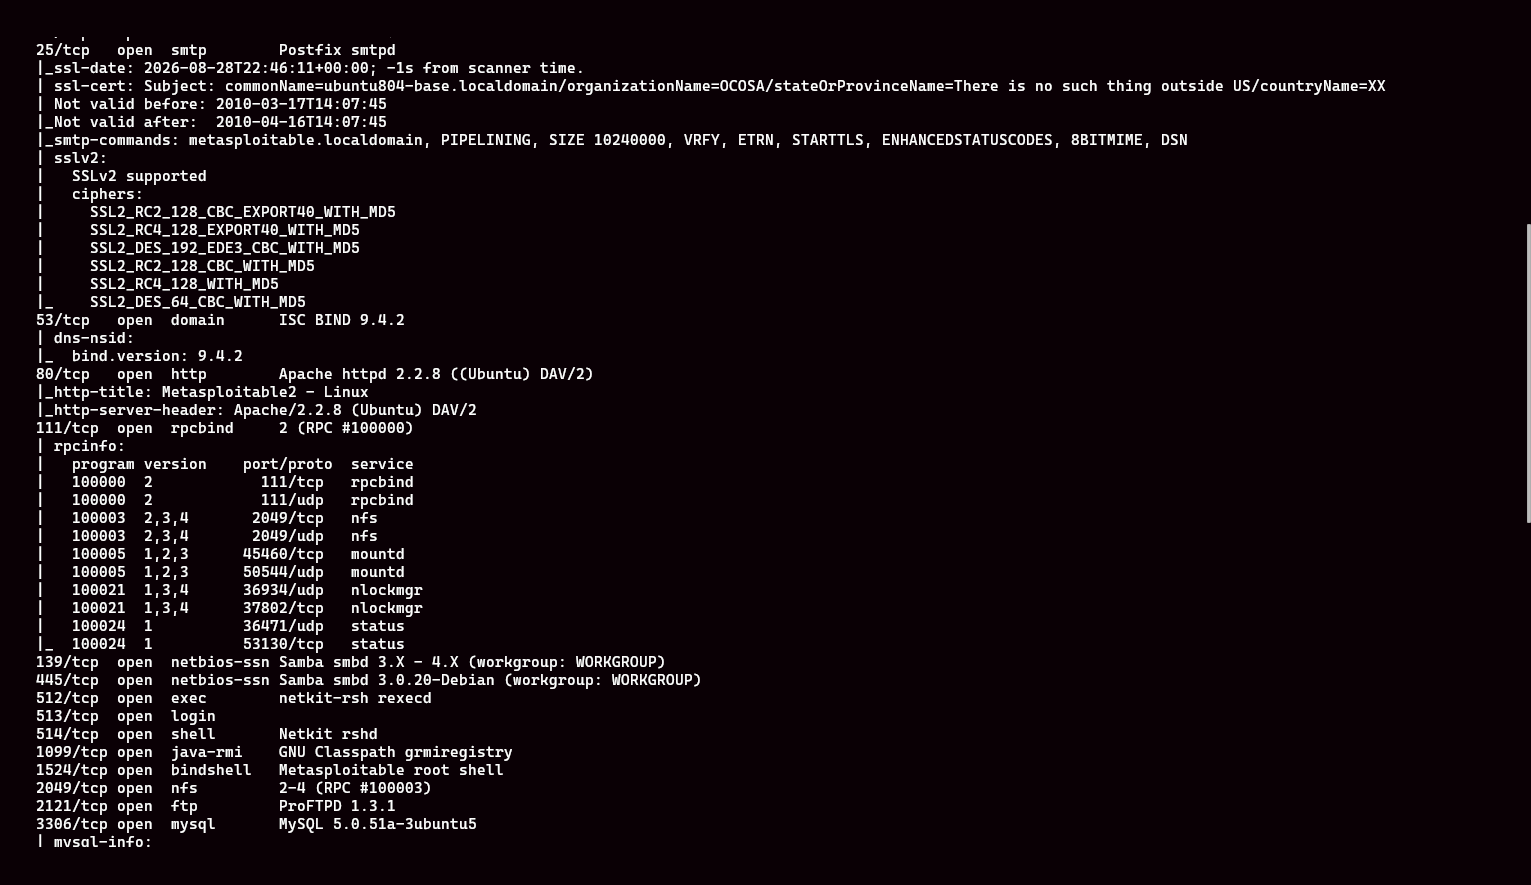
\includegraphics[width=\linewidth]{images/command2.png}
\end{evidence}

\begin{evidence}{3}{Aggressive scan continued --- ports 3306--8180 and host script results}
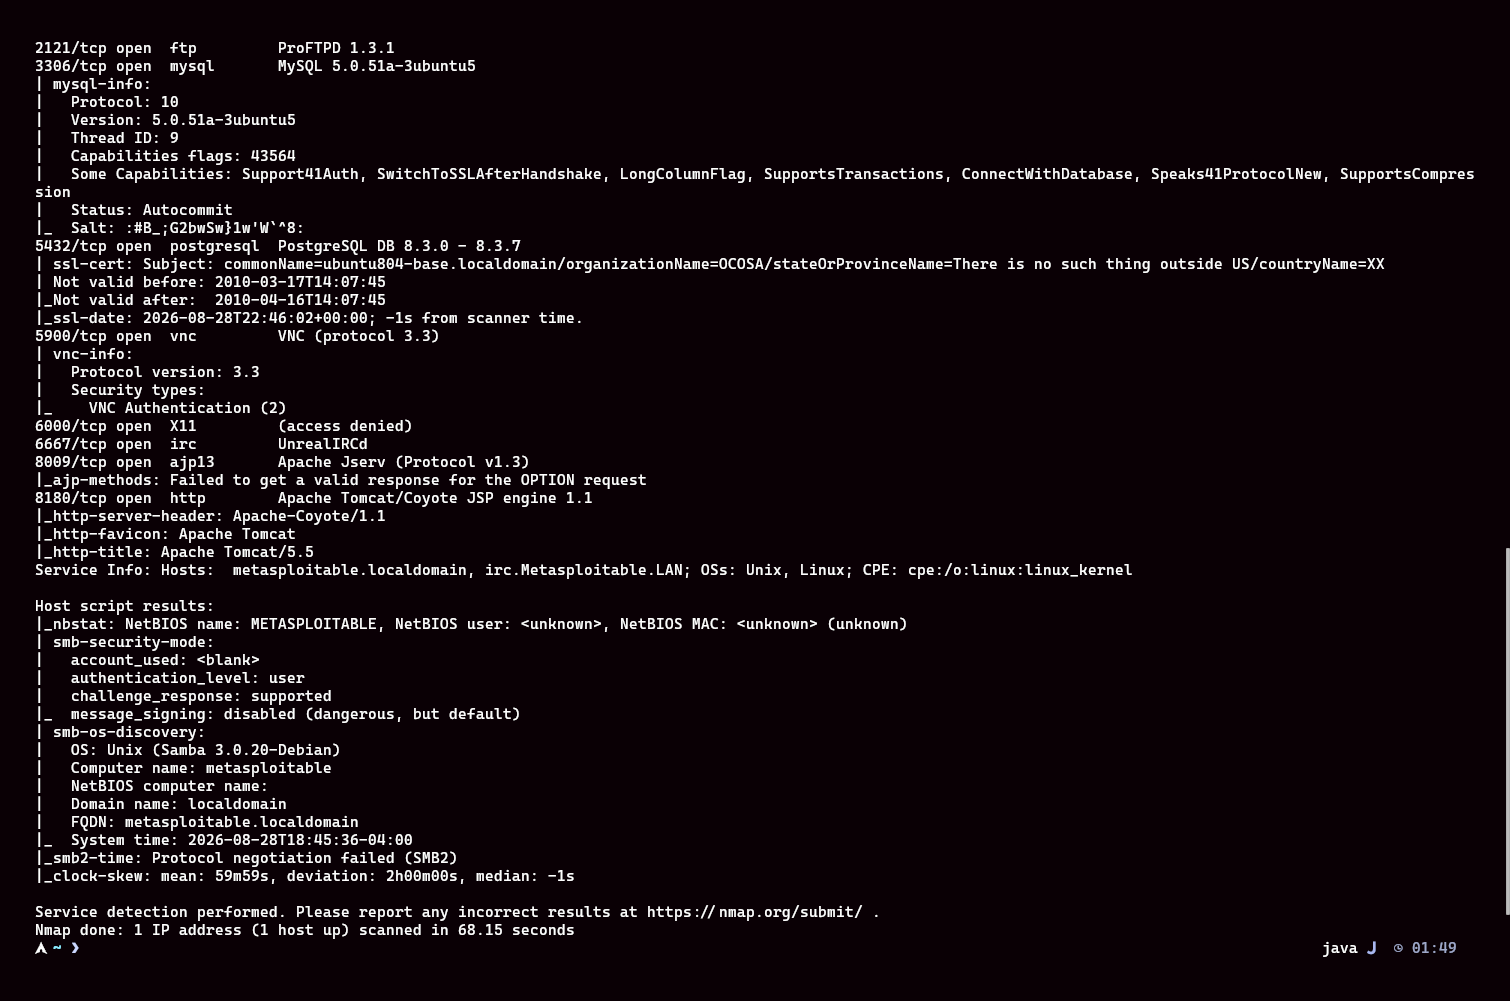
\includegraphics[width=\linewidth]{images/command3.png}
\end{evidence}

The scan completed in 68.15 seconds and returned 23 open TCP ports with service/version detection on all of them, plus SMB host-script output (OS fingerprint, security-mode, and clock-skew data) used in Section~7.

% ======================================================
\section{Hosts Identified}
% ======================================================

\begin{table}[h!]
\centering
\renewcommand{\arraystretch}{1.4}
\begin{tabular}{p{3.4cm} p{2.8cm} p{7cm}}
\toprule
\rowcolor{navy}
\textcolor{white}{\textbf{IP Address}} & \textcolor{white}{\textbf{Status}} & \textcolor{white}{\textbf{Role / Notes}} \\
\midrule
\texttt{192.168.56.1} & Up & Host-only virtual network gateway (hypervisor host) \\
\texttt{192.168.56.100} & Up & Secondary host on the lab subnet -- out of scope \\
\texttt{192.168.56.101} & Up & \textbf{Assessment target} -- Metasploitable2 \\
\bottomrule
\end{tabular}
\caption{Live hosts identified on \texttt{192.168.56.0/24}}
\end{table}

Only \texttt{192.168.56.101} was in scope for further enumeration and testing; the remaining two hosts were recorded for network-map completeness only.

% ======================================================
\section{Open Ports}
% ======================================================

\begin{longtable}{p{1.6cm} p{1.4cm} p{2.6cm} p{7.4cm}}
\toprule
\rowcolor{navy}
\textcolor{white}{\textbf{Port}} & \textcolor{white}{\textbf{State}} & \textcolor{white}{\textbf{Service}} & \textcolor{white}{\textbf{Version / Notes}} \\
\midrule
\endhead
21/tcp & open & ftp & vsftpd 2.3.4 (backdoored version) \\
22/tcp & open & ssh & OpenSSH 4.7p1 Debian 8ubuntu1 (protocol 2.0) \\
23/tcp & open & telnet & Linux telnetd (cleartext authentication) \\
25/tcp & open & smtp & Postfix smtpd \\
53/tcp & open & domain & ISC BIND 9.4.2 \\
80/tcp & open & http & Apache httpd 2.2.8 (Ubuntu) DAV/2 \\
111/tcp & open & rpcbind & RPC \#100000 (v2) \\
139/tcp & open & netbios-ssn & Samba smbd 3.X--4.X \\
445/tcp & open & netbios-ssn & Samba smbd 3.0.20-Debian \\
512/tcp & open & exec & netkit-rsh rexecd \\
513/tcp & open & login & rlogin \\
514/tcp & open & shell & Netkit rshd \\
1099/tcp & open & java-rmi & GNU Classpath grmiregistry \\
1524/tcp & open & bindshell & \textbf{Metasploitable root shell} (pre-existing backdoor) \\
2049/tcp & open & nfs & NFS 2--4 (RPC \#100003) \\
2121/tcp & open & ftp & ProFTPD 1.3.1 \\
3306/tcp & open & mysql & MySQL 5.0.51a-3ubuntu5 \\
5432/tcp & open & postgresql & PostgreSQL DB 8.3.0--8.3.7 \\
5900/tcp & open & vnc & VNC protocol 3.3 \\
6000/tcp & open & X11 & Access denied \\
6667/tcp & open & irc & UnrealIRCd \\
8009/tcp & open & ajp13 & Apache JServ Protocol v1.3 \\
8180/tcp & open & http & Apache Tomcat/Coyote JSP engine 1.1 \\
\bottomrule
\caption{Open ports and detected service versions on \texttt{192.168.56.101}}
\end{longtable}

% ======================================================
\section{Services Discovered}
% ======================================================

This section captures the enumeration and validation performed against the highest-value services identified above, with supporting evidence.

\subsection{FTP -- vsftpd 2.3.4 (Backdoor Validation)}
The detected vsftpd version corresponds to a publicly known trojaned release. Metasploit was used to confirm the presence of the matching exploit module.

\begin{evidence}{4}{Locating and selecting the vsftpd backdoor module in Metasploit}
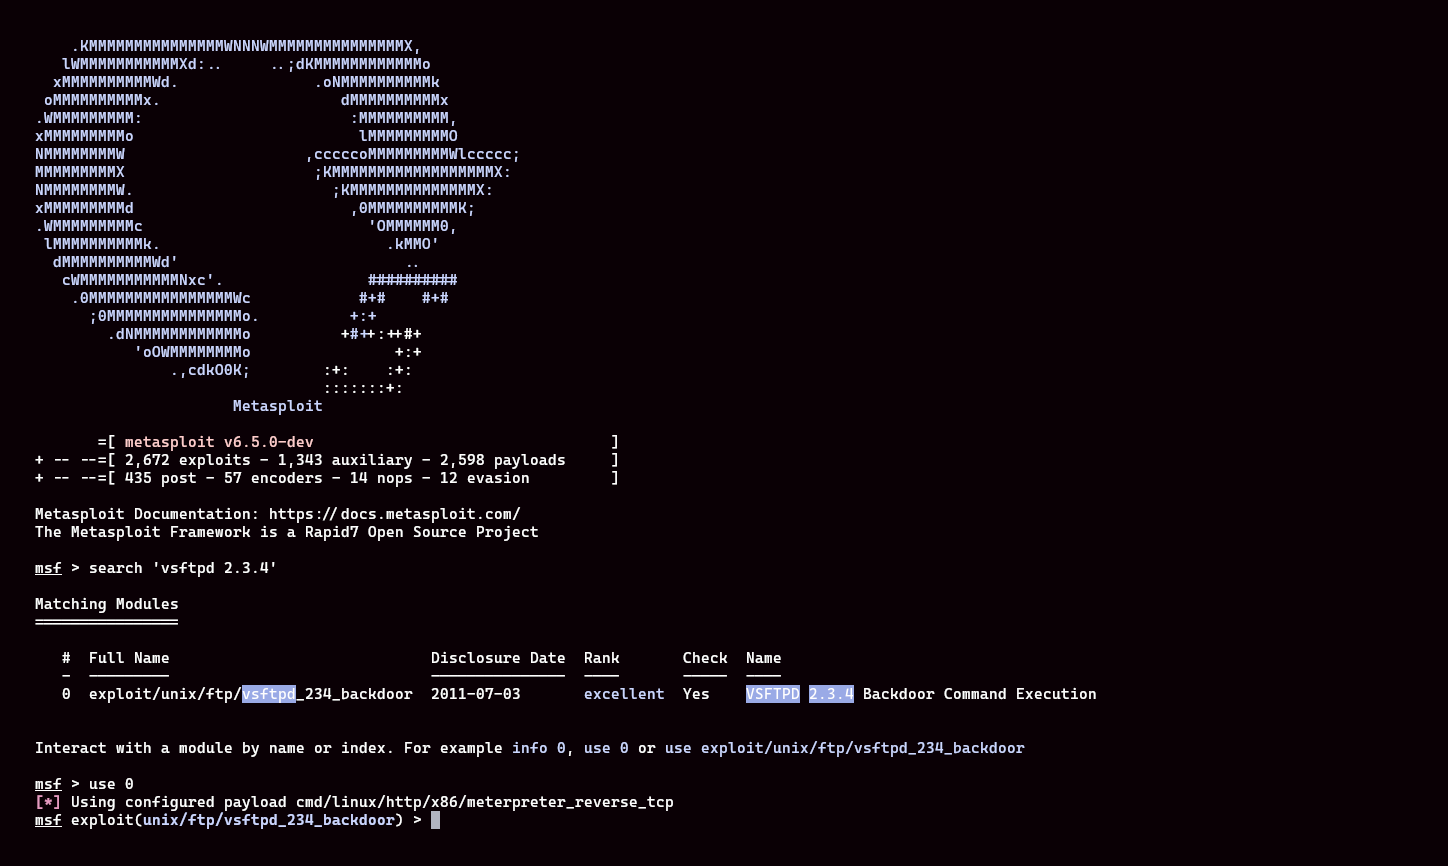
\includegraphics[width=\linewidth]{images/command4.png}
\end{evidence}

The module \texttt{exploit/unix/ftp/vsftpd\_234\_backdoor} matched exactly, confirming the target is running the compromised vsftpd 2.3.4 build. Combined with anonymous FTP login being permitted (see Section~7), this is one of the most severe findings in the assessment. \sev{4} -- see CVE-2011-2523 in Section~8.

\subsection{SSH -- OpenSSH 4.7p1}
SSH enumeration was performed using Metasploit's \texttt{ssh\_enumusers} auxiliary module against a username wordlist.

\begin{evidence}{5}{SSH username enumeration --- \texttt{auxiliary/scanner/ssh/ssh\_enumusers}}
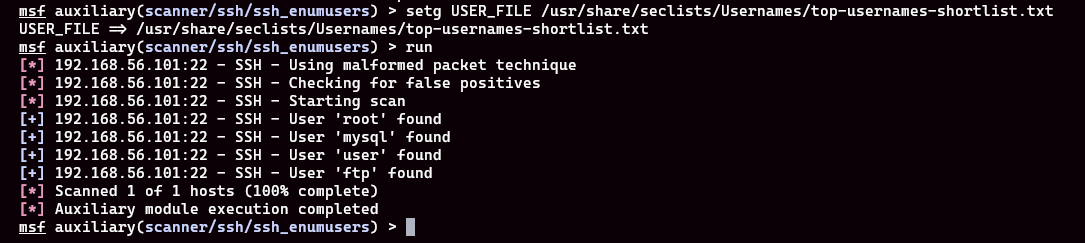
\includegraphics[width=\linewidth]{images/command5.png}
\end{evidence}

Four valid usernames were confirmed on the target: \texttt{root}, \texttt{mysql}, \texttt{user}, and \texttt{ftp}. Metasploit's \texttt{ssh\_version} scanner was then used to fingerprint the exact protocol/cipher configuration:

\begin{evidence}{6}{SSH version and algorithm fingerprinting --- \texttt{auxiliary/scanner/ssh/ssh\_version}}
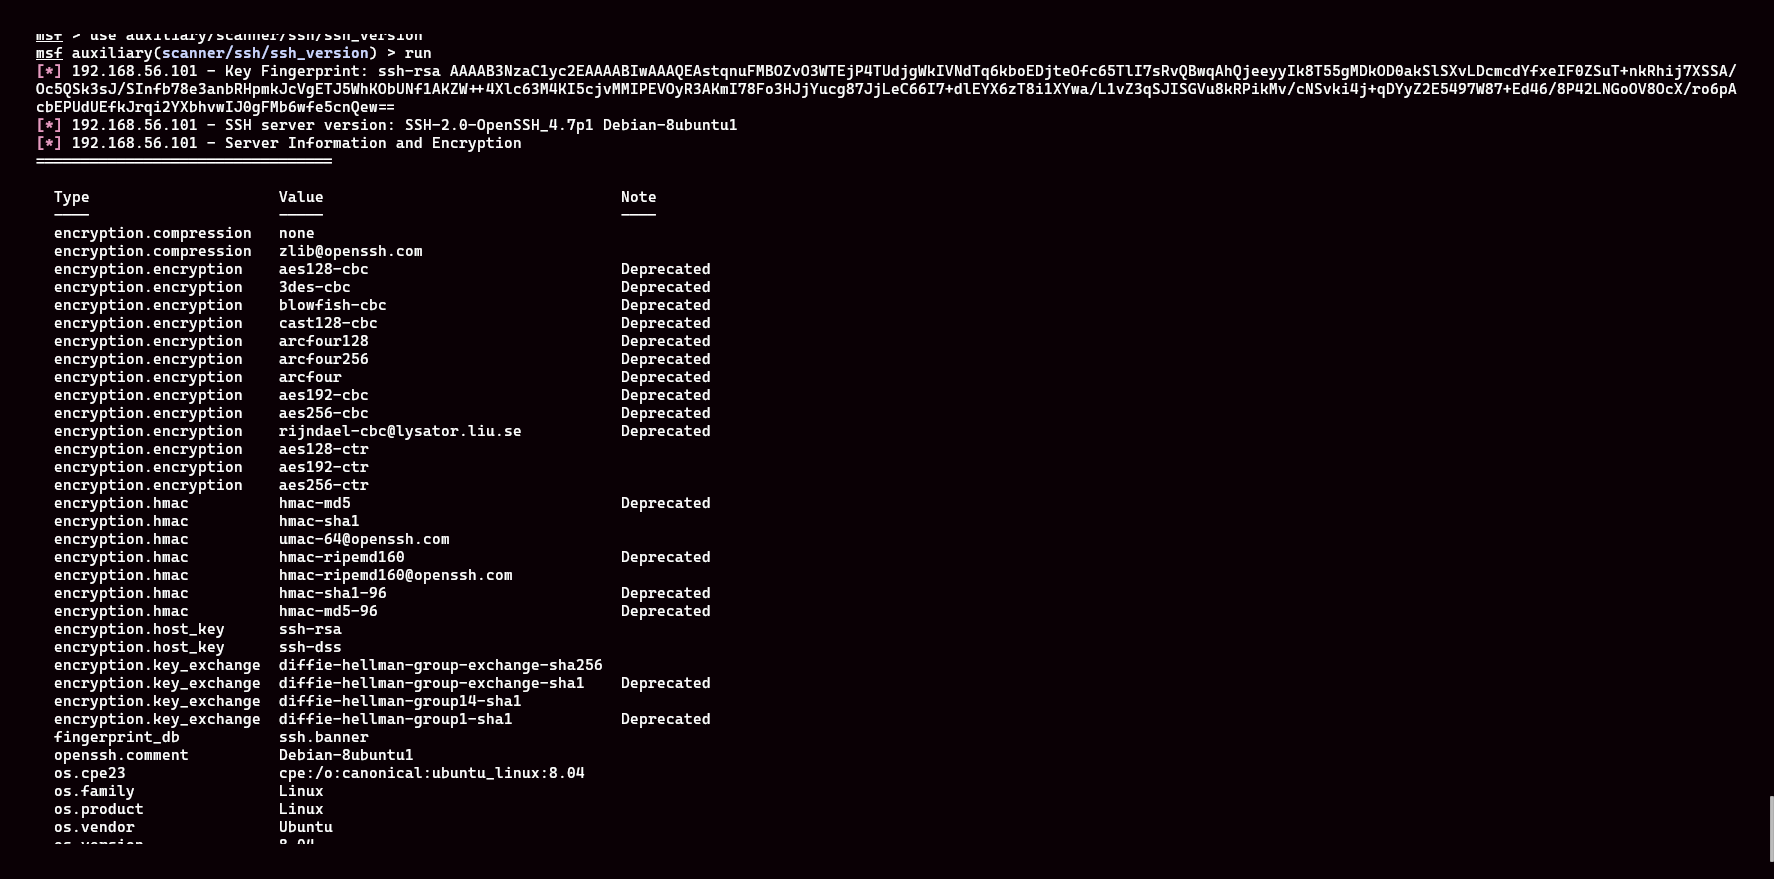
\includegraphics[width=\linewidth]{images/command6.png}
\end{evidence}

The server negotiates several deprecated ciphers and MAC algorithms (\texttt{arcfour}, \texttt{cbc}-mode ciphers, \texttt{hmac-md5}), consistent with OpenSSH 4.7p1's age. \sev{2} -- see CVE-2008-5161 in Section~8.

\subsection{Telnet}
Telnet exposes an unencrypted remote-administration channel. Metasploit's telnet version scanner was used to confirm the service banner.

\begin{evidence}{7}{Telnet service fingerprinting --- \texttt{auxiliary/scanner/telnet/telnet\_version}}
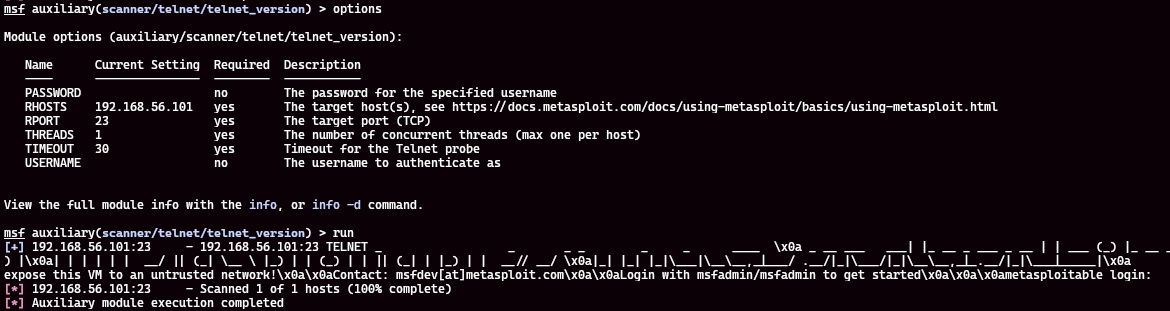
\includegraphics[width=\linewidth]{images/command10.png}
\end{evidence}

The banner confirms the standard Metasploitable2 login prompt and default-credential hint (\texttt{msfadmin/msfadmin}), and confirms that all telnet traffic -- including credentials -- is transmitted in cleartext. \sev{3}

\subsection{SMTP -- Postfix}
User enumeration via \texttt{VRFY}/\texttt{RCPT} was performed against the mail service using \texttt{smtp-user-enum}.

\begin{evidence}{8}{SMTP user enumeration --- \texttt{smtp-user-enum -m RCPT}}
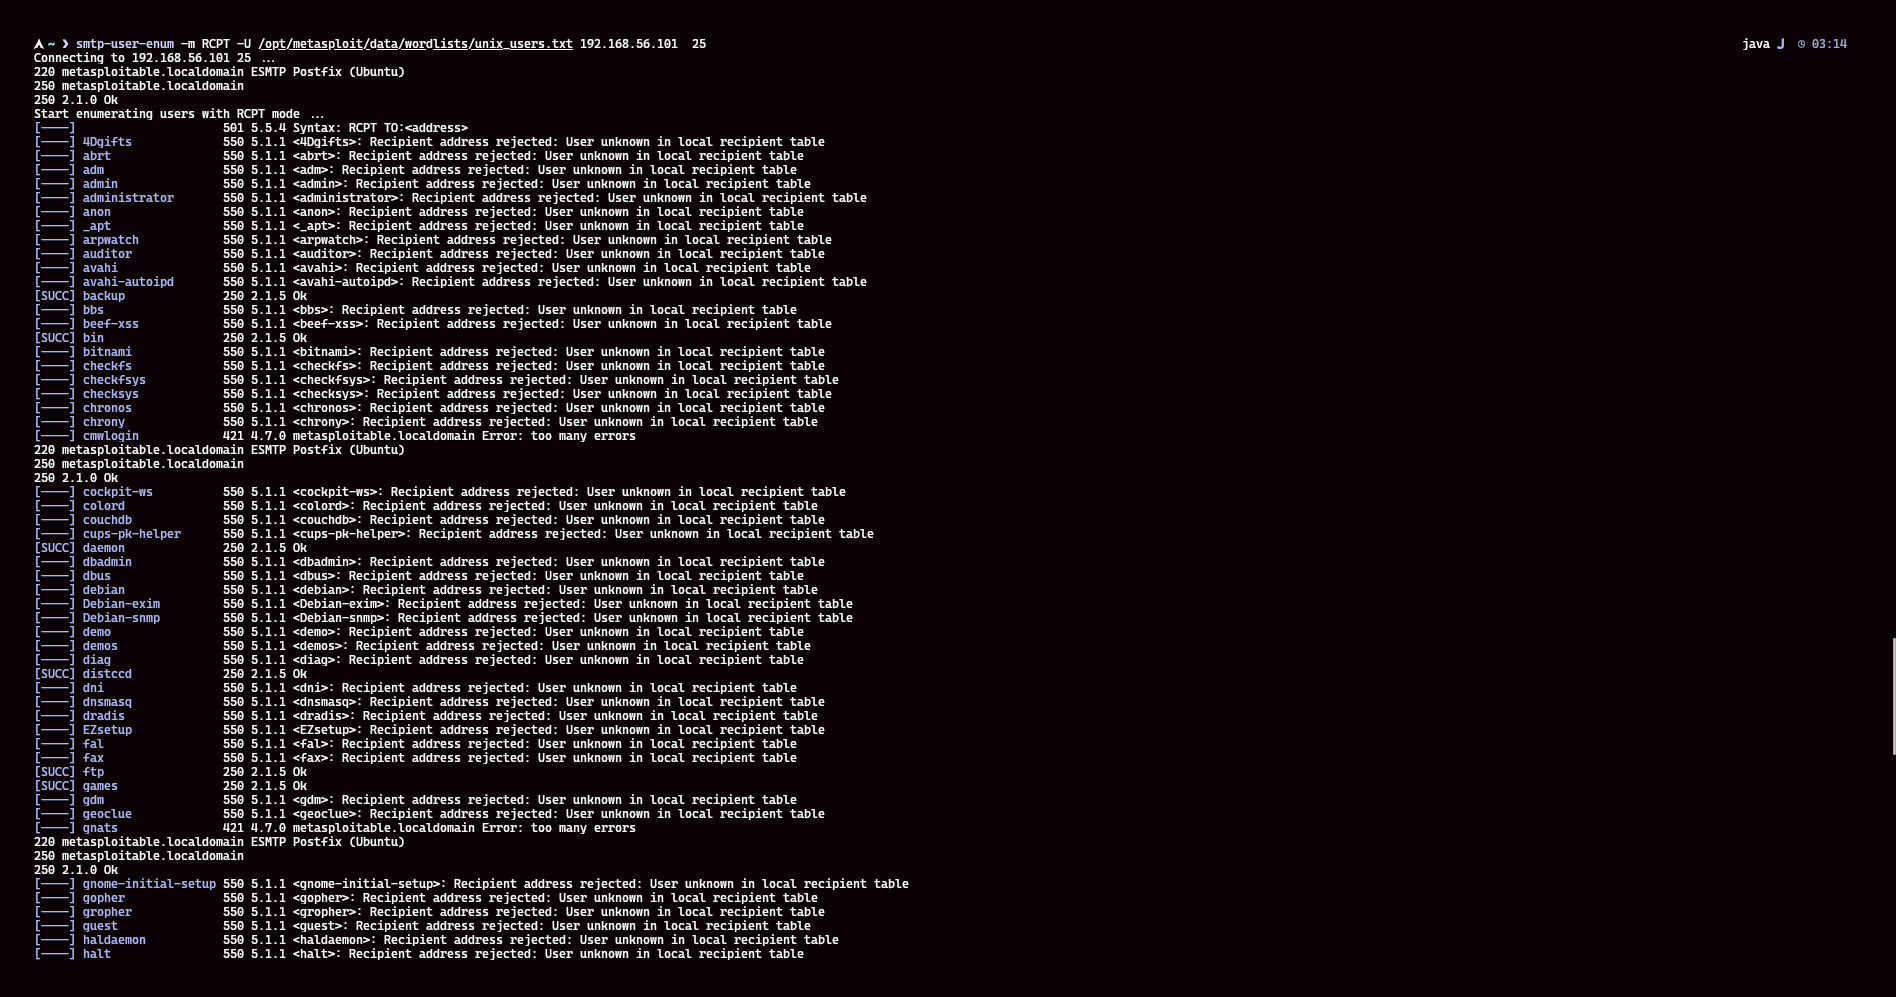
\includegraphics[width=\linewidth]{images/command11.png}
\end{evidence}

The SMTP service returned distinguishable ``250 2.1.5 Ok'' / ``550 5.1.1 \dots User unknown'' responses, allowing enumeration of valid local system accounts (\texttt{backup}, \texttt{bin}, \texttt{daemon}, \texttt{dbadmin}, \texttt{distccd}, \texttt{ftp}, \texttt{games}, \texttt{gdm}, and others). \sev{2}

% ======================================================
\section{Exploitation and Credential Attacks}
% ======================================================

\subsection{SSH Brute-Force Attacks}
Two independent brute-force attempts were performed against the SSH service using \texttt{nmap}'s \texttt{ssh-brute} NSE script.

\begin{evidence}{9}{Large-scale SSH brute force (SecLists wordlists, 601s runtime)}
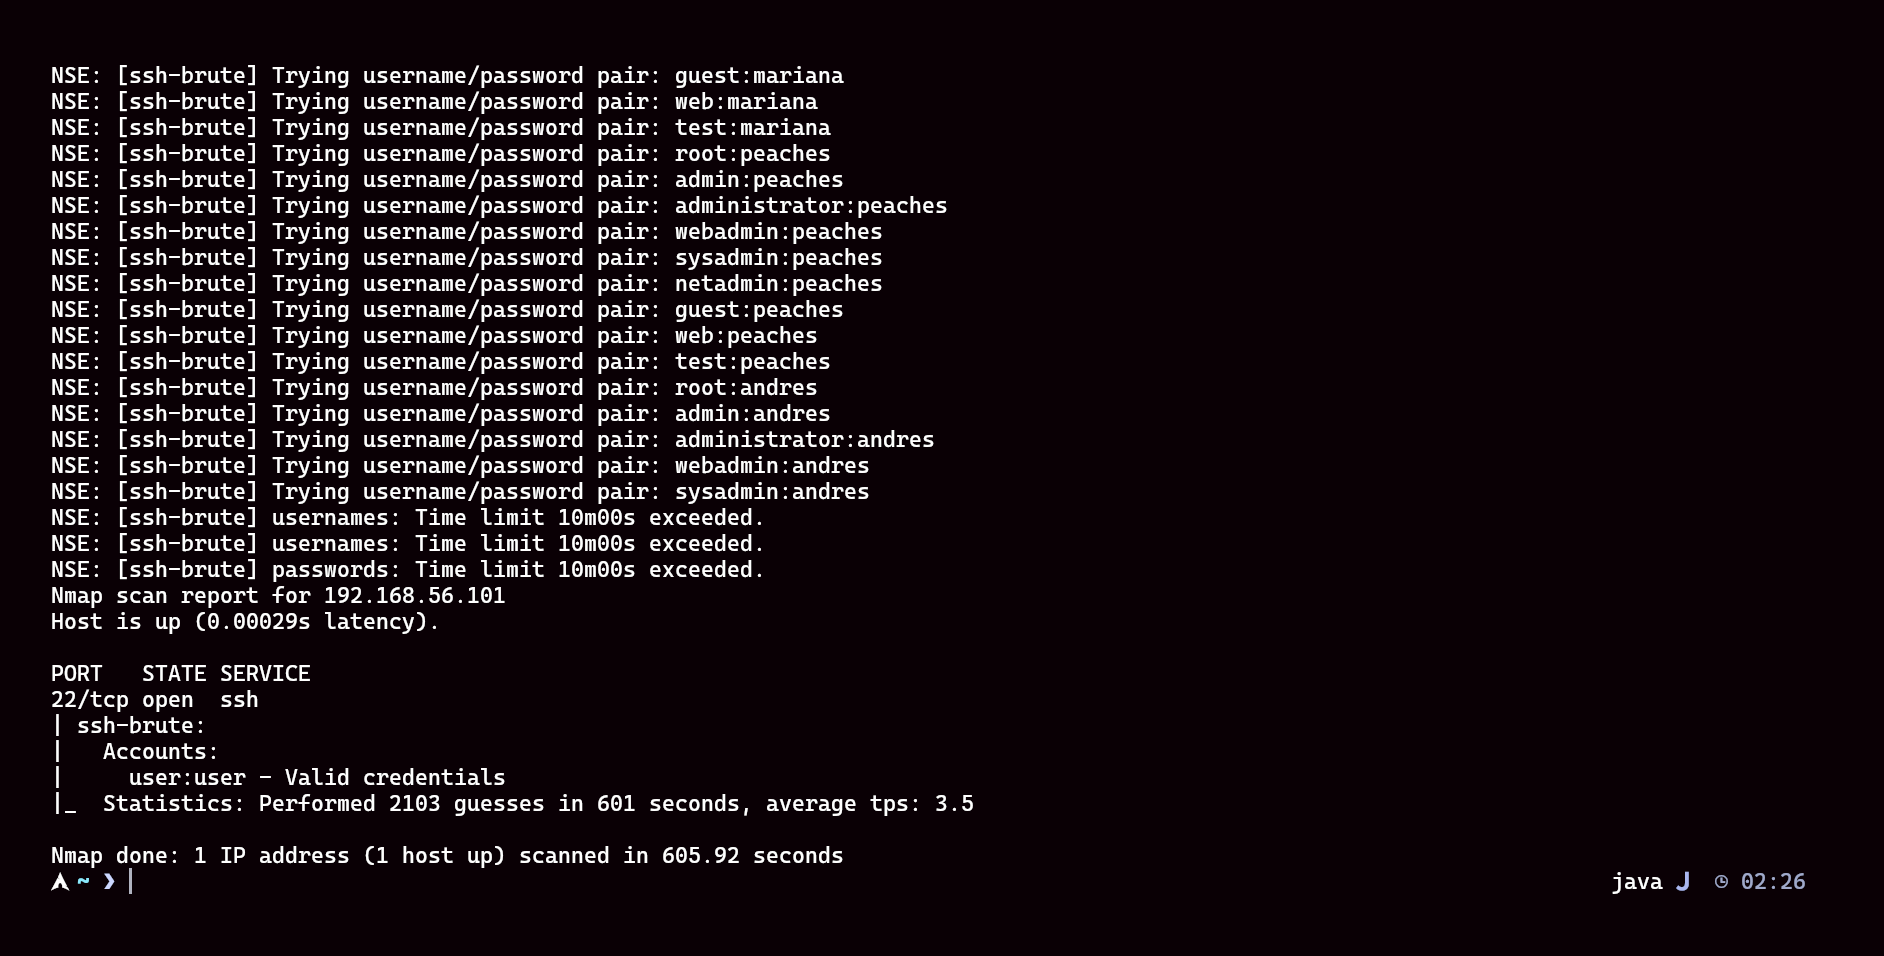
\includegraphics[width=\linewidth]{images/command7.png}
\end{evidence}

This run recovered valid credentials \texttt{user:user} after performing 2{,}103 password guesses in 601 seconds. A second, targeted run against the well-known default Metasploitable2 account was also successful:

\begin{evidence}{10}{Targeted SSH brute force against the default lab account}
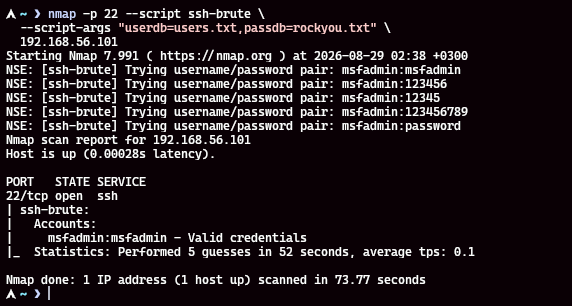
\includegraphics[width=\linewidth]{images/command9.png}
\end{evidence}

This confirmed \texttt{msfadmin:msfadmin} as a valid, weak, default credential pair -- the well-known intentional backdoor account shipped with Metasploitable2. \sev{4}

\subsection{Post-Authentication Evidence}
After authenticating as \texttt{user}, shell history was reviewed to illustrate what an attacker could observe and abuse after initial access.

\begin{evidence}{11}{Command history captured from an authenticated \texttt{user} session}
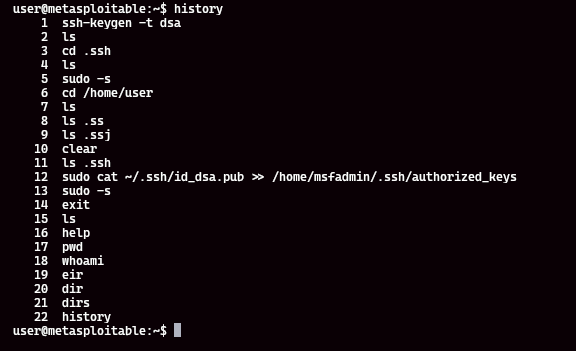
\includegraphics[width=\linewidth]{images/command8.png}
\end{evidence}

The history shows a prior operator generating an SSH keypair and appending the public key to \texttt{/home/msfadmin/.ssh/authorized\_keys} using \texttt{sudo}, along with repeated \texttt{sudo -s} invocations. This demonstrates how weak account hygiene and permissive \texttt{sudo} access on this host would let an attacker pivot from a low-privileged account to the \texttt{msfadmin} account, and highlights that command history is a valuable source of post-exploitation intelligence. \sev{3}

% ======================================================
\section{Potential Misconfigurations}
% ======================================================

\begin{itemize}[leftmargin=1.4em, itemsep=0.5em]
\item \textbf{Anonymous FTP login allowed} (port 21) -- the vsftpd service accepts anonymous logins (FTP code 230), exposing the file store to unauthenticated users.
\item \textbf{Cleartext protocols in use} -- FTP control/data, Telnet, and rsh/rlogin/rexec (ports 512--514) all transmit credentials and data unencrypted, allowing trivial network interception.
\item \textbf{SMB message signing disabled} -- \texttt{smb-security-mode} reports \texttt{message\_signing: disabled (dangerous, but default)}, permitting man-in-the-middle SMB relay attacks.
\item \textbf{Self-signed, expired SSL certificates} -- the SMTP and PostgreSQL services present a self-signed certificate for \texttt{ubuntu804-base.localdomain} that expired in April 2010, and both also expose legacy \texttt{SSLv2} with export-grade (40-bit) ciphers.
\item \textbf{Deprecated SSH ciphers/MACs} -- OpenSSH 4.7p1 negotiates CBC-mode ciphers, \texttt{arcfour}, and \texttt{hmac-md5}, all considered weak by modern standards.
\item \textbf{Weak/default credentials} -- both a generic weak password (\texttt{user:user}) and the well-known default lab credential (\texttt{msfadmin:msfadmin}) were valid on SSH.
\item \textbf{Excessive service exposure} -- NFS, rpcbind, X11, VNC, and a pre-existing root-level bindshell (port 1524) are all reachable from the network with no apparent access control.
\item \textbf{Large clock skew} -- \texttt{clock-skew: mean 59m59s, deviation 2h00m00s} was reported, which would undermine time-based authentication controls (e.g. Kerberos, TOTP) if deployed.
\end{itemize}

% ======================================================
\section{Relevant CVEs}
% ======================================================

\begin{longtable}{p{2.6cm} p{4.3cm} p{1.5cm} p{8cm}}
\toprule
\rowcolor{navy}
\textcolor{white}{\textbf{CVE ID}} & \textcolor{white}{\textbf{Affected Component}} & \textcolor{white}{\textbf{CVSS}} & \textcolor{white}{\textbf{Summary}} \\
\midrule
\endhead
CVE-2011-2523 & vsftpd 2.3.4 (port 21) & \textbf{9.8} (v3) / 10.0 (v2) & Trojaned source archive opens a root shell on TCP/6200 when a crafted username is supplied. Confirmed exploitable via \texttt{exploit/unix/ftp/vsftpd\_234\_backdoor}. \\
CVE-2010-2075 & UnrealIRCd (port 6667) & \textbf{10.0} (v2) & Trojaned source archive allows unauthenticated remote command execution via the \texttt{DEBUG3\_DOLOG\_SYSTEM} macro. \\
CVE-2007-2447 & Samba 3.0.20 (ports 139/445) & \textbf{6.0} (v2) & \texttt{usermap\_script} option allows remote command execution via shell metacharacters in MS-RPC calls. \\
CVE-2008-5161 & OpenSSH 4.7p1 (port 22) & \textbf{4.3} (v2) & CBC-mode cipher error handling can leak plaintext bits from ciphertext blocks in an SSH session. \\
CVE-2008-1447 & ISC BIND 9.4.2 (port 53) & \textbf{5.0} (v2) & ``Kaminsky bug'' -- weak transaction ID/source-port randomisation enables DNS cache-poisoning via birthday attacks. \\
CVE-2008-0122 & ISC BIND 9.4.2 (port 53) & \textbf{5.0} (v2) & Off-by-one error in \texttt{inet\_network()} can cause a crash (DoS) or memory corruption. \\
CVE-2009-4022 & ISC BIND 9.4.2 (port 53) & \textbf{5.0} (v2) & Flaw in DNSSEC validation of additional response-section records permits cache poisoning. \\
\bottomrule
\caption{CVEs mapped to identified service versions}
\end{longtable}

\begin{panel}
\small\textit{Note: CVSS scores above reflect the publicly documented base scores for each CVE as recorded by NVD/vendor advisories at the time of writing, and describe the vulnerability class in general -- not a re-scoring specific to this lab environment.}
\end{panel}

% ======================================================
\section{Recommendations}
% ======================================================

\begin{recbox}{Priority 1 --- Critical, remediate immediately}
\begin{itemize}[leftmargin=1.2em]
\item Remove/replace vsftpd 2.3.4 with a current, non-backdoored release; audit the FTP install path for signs of compromise.
\item Disable or replace UnrealIRCd; if IRC is required, deploy a current, verified-checksum build.
\item Remove the pre-existing root bindshell on port 1524 and audit the host for other unauthorized listeners.
\item Rotate and enforce strong, unique credentials for all accounts, especially \texttt{msfadmin} and \texttt{user}; disable password-only SSH authentication in favour of key-based auth.
\end{itemize}
\end{recbox}

\vspace{0.6em}
\begin{recbox}{Priority 2 --- High, remediate soon}
\begin{itemize}[leftmargin=1.2em]
\item Disable anonymous FTP access and restrict FTP to authenticated, least-privilege accounts.
\item Disable Telnet, rsh, rlogin, and rexec; replace with SSH for all remote administration.
\item Patch or reconfigure Samba to remove/disable the \texttt{username map script} option (CVE-2007-2447) and enable SMB message signing.
\item Upgrade BIND to a current release and enable DNSSEC/source-port randomisation to mitigate cache-poisoning risks.
\end{itemize}
\end{recbox}

\vspace{0.6em}
\begin{recbox}{Priority 3 --- Medium, plan for remediation}
\begin{itemize}[leftmargin=1.2em]
\item Upgrade OpenSSH and disable CBC-mode ciphers, \texttt{arcfour}, and MD5-based MACs in \texttt{sshd\_config}.
\item Replace expired self-signed certificates on SMTP/PostgreSQL and disable SSLv2 and export-grade ciphers.
\item Restrict or firewall exposure of NFS, rpcbind, X11, and VNC to trusted management networks only.
\item Correct system clock synchronisation (NTP) to eliminate the observed clock skew.
\end{itemize}
\end{recbox}

\vspace{0.6em}
\begin{recbox}{Priority 4 --- General hardening}
\begin{itemize}[leftmargin=1.2em]
\item Implement network segmentation so this class of legacy service is never reachable from untrusted networks.
\item Enable centralized logging and alerting for authentication failures and brute-force patterns (e.g. \texttt{fail2ban} or an IDS).
\item Establish a periodic vulnerability-scanning cadence to catch reintroduced legacy packages.
\end{itemize}
\end{recbox}

% ======================================================
\section*{Appendix A -- Tools Used}
\addcontentsline{toc}{section}{Appendix A -- Tools Used}
% ======================================================

\begin{table}[h!]
\centering
\renewcommand{\arraystretch}{1.3}
\begin{tabular}{p{3.6cm} p{9.5cm}}
\toprule
\rowcolor{navy}
\textcolor{white}{\textbf{Tool}} & \textcolor{white}{\textbf{Purpose}} \\
\midrule
Nmap 7.991 & Host discovery, port scanning, service/version detection, NSE scripts (\texttt{ssh-brute}) \\
Metasploit Framework 6.5.0-dev & Module search/exploitation validation, SSH user/version enumeration, Telnet version scanning \\
smtp-user-enum & SMTP account enumeration via RCPT/VRFY \\
SecLists & Username and password wordlists for brute-force testing \\
\bottomrule
\end{tabular}
\end{table}

\end{document}